%%  Math, Tables, and FIgures Template: Compiled by Kyle Davis
%    The Ohio State University
%       - For aid in writing math and tables in LaTeX.
%    This is minimalist; feel free to compile using: 
%! PDFLatex -> View PDF
%-----------------------------------------------------------
\documentclass[12pt]{article}

%! Some formatting tools: (\mathlarger)
\usepackage{graphicx, fullpage, natbib, float, relsize, epsfig} 
%! Math tools
\usepackage{amsfonts, amsmath, amsthm, amssymb, mathtools} 
% Set margins
\usepackage[top = 1in, left = 1in, right = 1in, bottom = 1in]{geometry}
\usepackage{setspace}
% Hides hyperlink red box.
\usepackage[bookmarks = false, hidelinks]{hyperref} 
% Aids float of tables/figures
\usepackage{float}
\usepackage{subcaption}

% Font Formatting (american):
\usepackage[compact]{titlesec}
\usepackage{baskervald} 
\usepackage[style = american]{csquotes}
\usepackage[american]{babel}

% Footnote Formatting
\usepackage{scrextend}
\usepackage{enumitem} %Footnote Formatting
\usepackage{listings} %Footnote Formatting

\setlist{nolistsep, noitemsep}
\setlength{\footnotesep}{1.2\baselineskip}
\deffootnote[.2in]{0in}{0em}{\normalsize\thefootnotemark.\enskip}

% Section Formatting 
\def\ci{\perp\!\!\!\perp}
\titleformat*{\section}{\large\bfseries}
\titleformat*{\subsection}{\normalsize\bfseries}

% To insert graphics using:: \includegraphics[scale=�]{�}
\usepackage{graphicx}
%\graphicspath{{ directory location of image }}

%! Used in making graphs and plotting:
\usepackage{tikz}
\usetikzlibrary{positioning}
\usepackage{tkz-graph}
\usetikzlibrary{shapes,arrows}
\usepackage{caption}
\newcommand*{\h}{\hspace{5pt}}% for indentation
\newcommand*{\hh}{\h\h}       % double indentation

%---------------------------------------------------------
\pagestyle{plain}
\begin{document}
% Comment this (%) if you prefer indents: 
\setlength{\parindent}{0pt}
\setcounter{page}{1}
\singlespacing 

%------------------- Document Conten ---------------------
% Header:
\begin{center}
\textbf{The Wonderful and Wacky World of Math!}\\
https://github.com/KyleDavisGithub
\end{center}
% Double spaced content:
% \doublespacing
\textbf{Introduction: Basic Concepts}

Math is great and all but how can we make math look great in \LaTeX ? Isn't most of it as simple as $1+1$? Well no, we can have it separated:

$$ 1+1 $$

or noted off to the side for reference (See equation 1).

\begin{equation}
1+1
\end{equation}

From here we can expand and express anything mathematically! I've listed a ton of examples below on formatting that should help with a lot of different scenarios.

\hfill 

\textbf{Common Math Equations:}

% Greek:
\textit{Basic Linear Model}
\begin{equation}
\mathlarger{ y = \beta_0 + \beta X + \epsilon }
\end{equation}

% Fractions:
\textit{z Score Formula}
\begin{equation}
z_i = \frac{x_i - \bar{x}}{s} = z = \frac{x - \mu}{\sigma}
\end{equation}

% Square Root:
\textit{T-score}
\begin{equation}
t = \frac{X-\mu}{\frac{s}{\sqrt{(n)}}}
\end{equation}

% Subscript and Superscript:
\textit{Error Assumption Equation}
\begin{equation}
\mathlarger{  \epsilon_i  \thicksim \mathcal{N}(0, \sigma^2)     }
\end{equation}

% mean (\bar) and having both sub/super scripts. 
\textit{Calculating Explained Variance}
\begin{equation}
\mathlarger{ \text{R}^2 = 1 - \frac{\text{RSS}}{\text{TSS}} = \frac{\Sigma \epsilon^{2}_i}{\Sigma\left(Y_i - \bar{Y}\right)^2}          }
\end{equation}

% Classifying cases, having text.
\textit{Logit and Probit}
\begin{equation}\nonumber
\text{Logit/Probit DV} 
\begin{cases}
  1 = \text{for event occuring}    \\
  0 = \text{for event not occuring} 
\end{cases}
\end{equation}

% Text and upper-case greek.
\begin{equation}
\text{logit:  } \eta =  p\left( \frac{p}{1-p}\right)  
\end{equation}
\begin{equation}
\text{probit:  } \eta = \Phi^{-1}(p) \text{where }  \Phi^{-1} \text{ is the inverse normal distribution CDF}
\end{equation}

\begin{equation}
\text{logit}^{-1} (\eta_i) = \frac{e^{\eta_i}}{1+e^{\eta_i}} \text{ to or from: } \eta_i = p\left( \frac{p}{1-p}\right) 
\end{equation}

\textit{Poisson PDF}
\begin{equation}
\mathlarger{ \frac{\lambda^k e^{-\lambda}}{k!}     }
\end{equation}

\textit{AIC and BIC}
\begin{equation}
AIC = -2 \ln L(\hat{\theta} \vert y) + 2p = D(\hat{\theta} ) +2p 
\end{equation}

\begin{equation}
BIC = -2 \ln L(\hat{\theta} \vert x) +plog(n) = D(\hat{\theta}) + p \ln (n)
\end{equation}

\textit{Inverse Logit Predicted Probabilities: Ordered Logit}
\begin{equation}
logit^{-1} (\theta_{k+1}) - logit^{-1}(\theta_k)
\end{equation}

\textit{Multinomial Link Function}
\begin{equation}
\eta_{ij} = x^{T}_i \beta_j = log \frac{p_{ij}}{p_{i1}} \hspace{.5cm} \forall  \hspace{.5cm}  j = 2, ... , J    
\end{equation}

\begin{equation}
 p_{ij} = \frac{exp(\eta_{ij})}{1+ \Sigma^{J}_{j=2} exp (\eta_{ij})   }     
\end{equation}

% Including how to not number: sections:
\textit{Types of Machine Learning} 
\begin{equation}\nonumber 
\begin{cases}
\text{Supervised learning} \begin{cases} \text{Classification} \\ \text{Regression} \end{cases}\\
\text{Unsupervised learning} \begin{cases} \text{Discovering clusters} \\ \text{Discovering latent factors} \\ \text{Discovering graph structure} \\ \text{Matrix completion} \end{cases}\\
\end{cases}
\end{equation}



%-------------------   Tables   --------------------------

\clearpage
\textbf{Tables}:

The following two examples are using R's \texttt{texreg} package. This R package will build \LaTeX~ code for tables depending on the model and code within R. That package's help file is useful in specifying the contents for the tables here, but we can change the tables within \LaTeX~ as well:

% Begin table, setting "float" position to "here!" 
\begin{table}[h!]
\caption{Model}
\begin{center}
\begin{tabular}{l c }             % 2 columns (1, and "c"). 
\hline                            % \hline just adds a line
           & $\hat{y}$         \\ % "&" separates columns
\hline
Intercept  & $2.09^{*}$        \\
           & $[2.09;\ 2.09]$   \\
$x_1$      & $-1.00^{*}$       \\
           & $[-1.00;\ -1.00]$ \\
$x_2$      & $2.99^{*}$        \\
           & $[2.99;\ 2.99]$   \\
\hline
R$^2$      & 0.88              \\
Adj. R$^2$ & 0.88              \\
Num. obs.  & 1000              \\
RMSE       & 2.04              \\
\hline
\multicolumn{2}{l}{\scriptsize{CI's Overridden by Bootstrap; [.05, .95]}}
\end{tabular}
\label{table:coefficients} 
% This label can be referenced in text
\end{center}
\end{table}


% Multiple Columns:
\begin{table}[h!]
\caption{Survival Modeling Duration}
\begin{center}
\begin{tabular}{l c c c }
\hline
 & Exponential & Weibull & exp(Cox) \\
\hline
Intercept          & $3.60$    & $3.59$    &           \\
                   & $(0.10)$  & $(0.10)$  &           \\
Investiture        & $-0.36$   & $-0.34$   &           \\
                   & $(0.13)$  & $(0.12)$  &           \\
Polarization       & $-0.039$  & $-0.04$   & $1.04$    \\
                   & $(0.01)$  & $(0.005)$ & $(0.01)$  \\
Crisis Duration    & $0.01$    & $0.01$    & $0.99$    \\
                   & $(0.002)$ & $(0.002)$ & $(0.002)$ \\
Log(Scale)         &           & $-0.12$   &           \\
                   &           & $(0.05)$  &           \\

\hline
Scale              & Fixed 1   & 0.884     &           \\
Log\ Likelihood    & -1056.7   & -1053.8   & 56.6      \\
$\chi^2$           & 88.08     & 93.6      &           \\
df                 &  3        &   3       & 2         \\
Num.\ obs.         & 314       & 314       & 314       \\
\hline
\multicolumn{4}{l}{\scriptsize{-}}
\end{tabular}
\end{center}
\end{table}

% clears page, similar to \newpage
\clearpage



%----------------- Figures -----------------------
\textbf{Graphs and Visualizations:}
%% These graphs are very usful to readers and to organize thoughts for yourself. If you're stuck on how to begin one of these (using tikz) consider shopping around online for something similar (Google is great):

% http://texample.net/tikz/examples/

% Here are some examples that should help:
\begin{center}
% The beginning tikzpicture [brackets] has the settings
% and functions for the rest of the graph, the graph will
% generate the nodes (the center connecting points) and
% the paths (the lines intersecting these nodes)

% more details on the measurements of these lines:
% https://tex.stackexchange.com/questions/8260/what-are-the-various-units-ex-em-in-pt-bp-dd-pc-expressed-in-mm
\begin{tikzpicture}[%
    ->,
    shorten >=2pt,
    >=stealth,
    node distance=3cm,
    noname/.style={%
      rectangle,
      minimum width=2em,
      minimum height=2em,
      draw
    }
  ]
  % Nodes: 
    \node[noname] (C)                                   {C};
    \node[noname] (D) [node distance=2cm, below right=of C] {D};
    \node[noname] (O) [right=of C]        				{O};
    \node[noname] (Y) [node distance=2cm, below right=of O] {Y};
  % Paths: 
    \path (D) edge     node {} (Y)
          (C) edge     node {} (D)
          (C) edge     node {} (O)
          (O) edge     node {} (Y);
\end{tikzpicture}
\end{center}

\hfill 

% https://tex.stackexchange.com/questions/45806/tikzpicture-how-can-i-draw-a-loop-right-below
\begin{center}
\begin{tikzpicture}[->,>=stealth',shorten >=1pt,thick]
\SetGraphUnit{3} 
\tikzset{VertexStyle/.style = {draw,rectangle,thick,
                               minimum size=1cm,
                               font=\large\bfseries},thick} 
\Vertex{1} \SOWE(1){2} \SOEA(1){3} 
\Edges(3,2,1) \Edge(3)(1)

\Loop[dist=2cm,dir=NO,label=$0.6$,labelstyle=above](1)  
\Loop[dist=2cm,dir=SOEA,label=$0.8$,labelstyle=below right](3)  

\path[every node/.style={swap,auto}]    (2) to node {0.1} (1)
                                            to node {0.1} (3)
                                            to node {0.1} (2); 
\draw[->] (1) to [bend right] node [above left] {0.4} (2);
% it's possible with \Edge but Tikz's syntax is allowed too.
\end{tikzpicture} 
\end{center}


\hfill 


% From:
% Author: Stefan Kottwitz
% https://www.packtpub.com/hardware-and-creative/latex-cookbook
\begin{center}
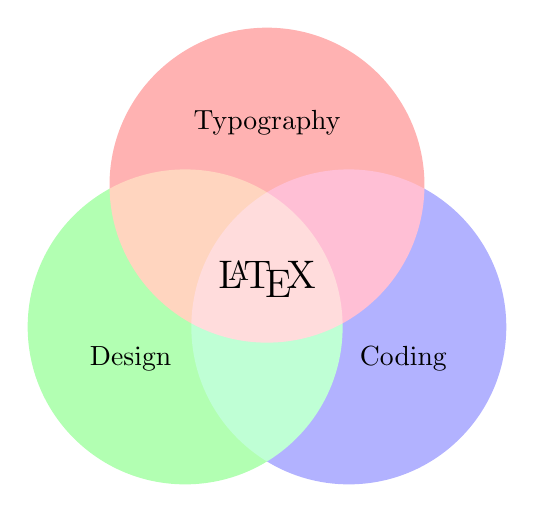
\begin{tikzpicture}
  \begin{scope}[blend group = soft light]
    \fill[red!30!white]   ( 90:1.2) circle (2);
    \fill[green!30!white] (210:1.2) circle (2);
    \fill[blue!30!white]  (330:1.2) circle (2);
  \end{scope}
  \node at ( 90:2)    {Typography};
  \node at ( 210:2)   {Design};
  \node at ( 330:2)   {Coding};
  \node [font=\Large] {\LaTeX};
\end{tikzpicture}
\end{center}




% A CONSORT-style flowchart of a randomized controlled trial
% using the PGF/TikZ package
% Author  : Morten Vejs Willert (July 2010)
% License : Creative Commons attribution license
\newpage
\begin{center}
  \textit{Flowchart of participants' progress through the phases of the trial}
  % setting the typeface to sans serif and the font size to small
  % the scope local to the environment
  \sffamily
  \footnotesize
  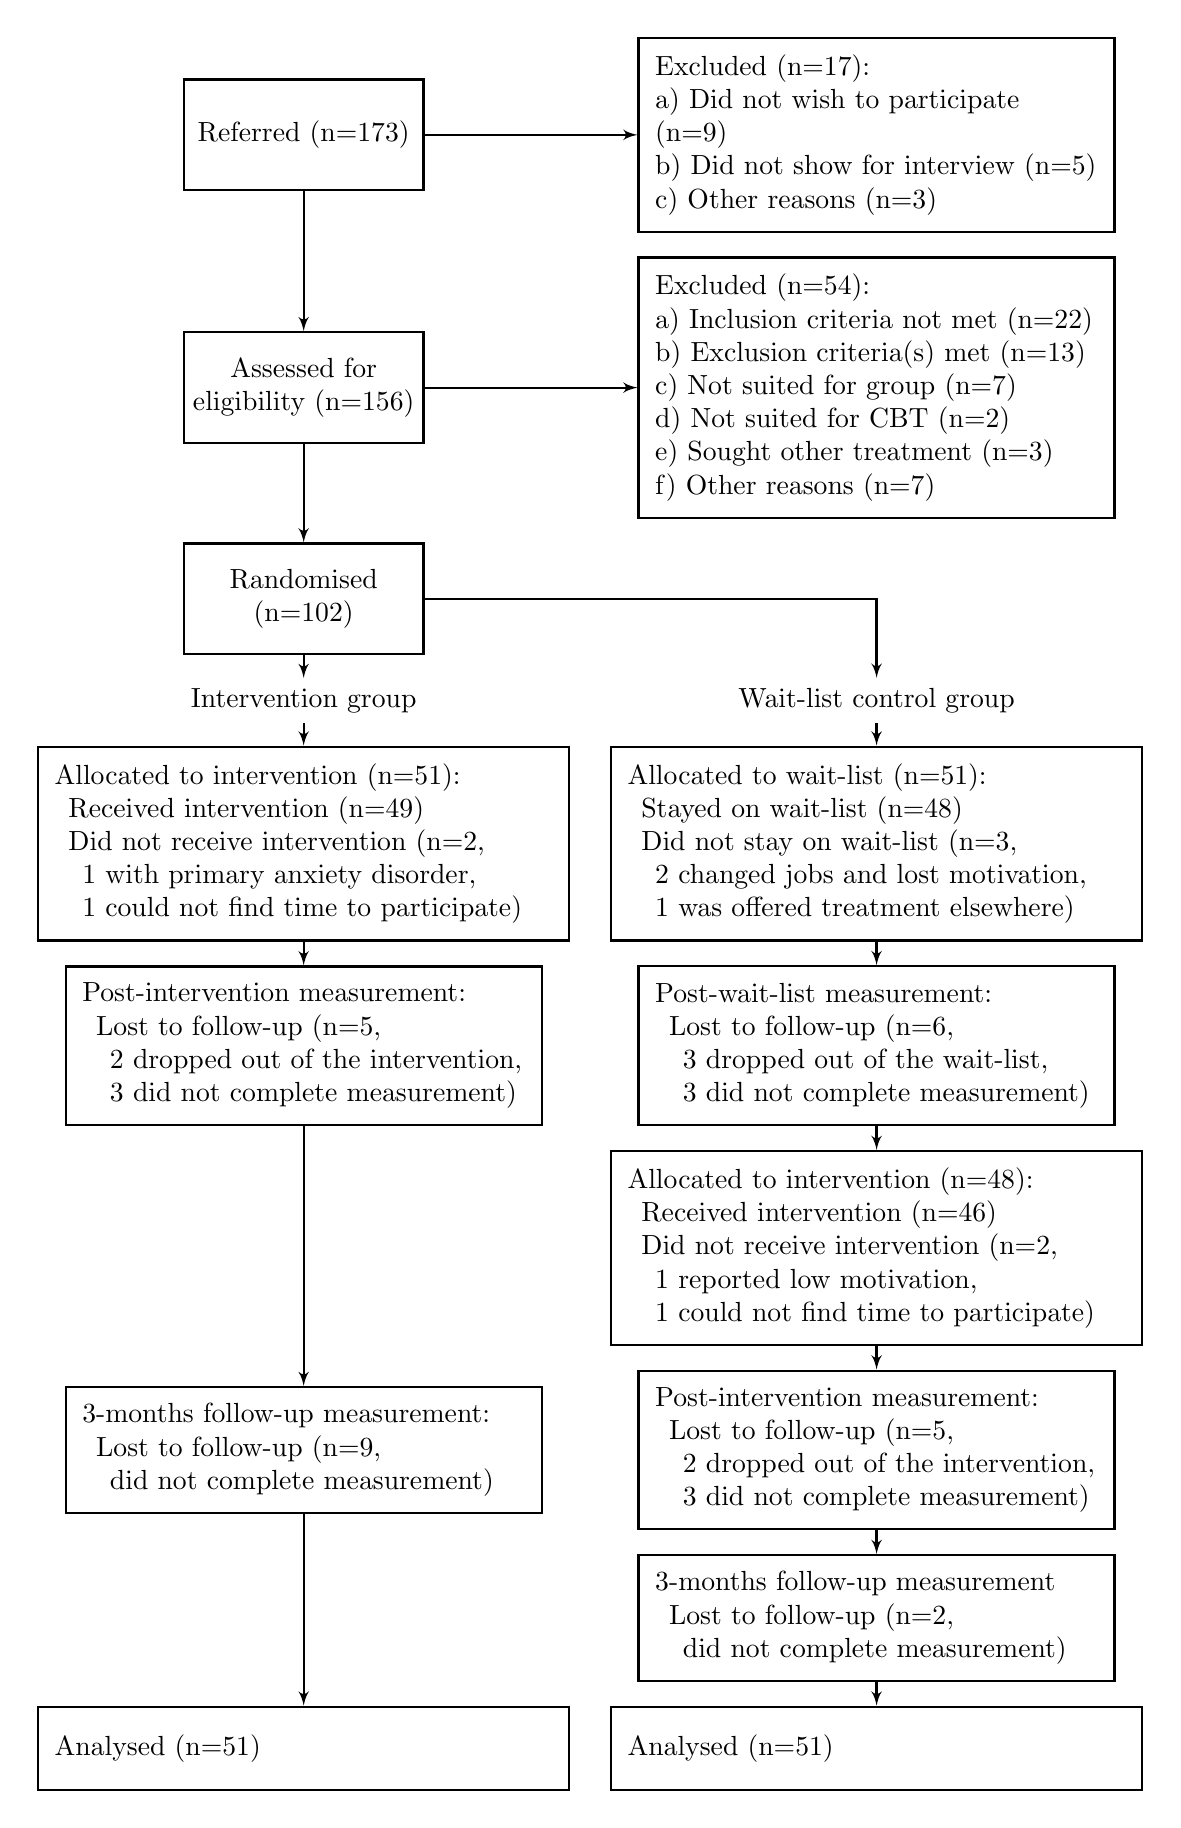
\begin{tikzpicture}[auto,
    %decision/.style={diamond, draw=black, thick, fill=white,
    %text width=8em, text badly centered,
    %inner sep=1pt, font=\sffamily\small},
    block_center/.style ={rectangle, draw=black, thick, fill=white,
      text width=8em, text centered,
      minimum height=4em},
    block_left/.style ={rectangle, draw=black, thick, fill=white,
      text width=16em, text ragged, minimum height=4em, inner sep=6pt},
    block_noborder/.style ={rectangle, draw=none, thick, fill=none,
      text width=18em, text centered, minimum height=1em},
    block_assign/.style ={rectangle, draw=black, thick, fill=white,
      text width=18em, text ragged, minimum height=3em, inner sep=6pt},
    block_lost/.style ={rectangle, draw=black, thick, fill=white,
      text width=16em, text ragged, minimum height=3em, inner sep=6pt},
      line/.style ={draw, thick, -latex', shorten >=0pt}]
    % outlining the flowchart using the PGF/TikZ matrix funtion
    \matrix [column sep=5mm,row sep=3mm] {
      % enrollment - row 1
      \node [block_center] (referred) {Referred (n=173)};
      & \node [block_left] (excluded1) {Excluded (n=17): \\
        a) Did not wish to participate (n=9) \\
        b) Did not show for interview (n=5) \\
        c) Other reasons (n=3)}; \\
      % enrollment - row 2
      \node [block_center] (assessment) {Assessed for eligibility (n=156)}; 
      & \node [block_left] (excluded2) {Excluded (n=54): \\
        a) Inclusion criteria not met (n=22) \\
        b) Exclusion criteria(s) met (n=13) \\
        c) Not suited for group (n=7) \\
        d) Not suited for CBT (n=2) \\
        e) Sought other treatment (n=3) \\
        f) Other reasons (n=7)}; \\
      % enrollment - row 3
      \node [block_center] (random) {Randomised (n=102)}; 
      & \\
      % follow-up - row 4
      \node [block_noborder] (i) {Intervention group}; 
      & \node [block_noborder] (wlc) {Wait-list control group}; \\
      % follow-up - row 5
      \node [block_assign] (i_T0) {Allocated to intervention (n=51): \\
      \h Received intervention (n=49) \\
      \h Did not receive intervention (n=2, \\
      \hh 1 with primary anxiety disorder, \\
      \hh 1 could not find time to participate)}; 
	  & \node [block_assign] (wlc_T0) {Allocated to wait-list (n=51): \\
      \h Stayed on wait-list (n=48) \\
      \h Did not stay on wait-list (n=3, \\
      \hh 2 changed jobs and lost motivation, \\
      \hh 1 was offered treatment elsewhere)}; \\
      % follow-up - row 6
      \node [block_lost] (i_T3) {Post-intervention measurement: \\
      \h Lost to follow-up (n=5, \\
      \hh 2 dropped out of the intervention, \\
      \hh 3 did not complete measurement)}; 
	  & \node [block_lost] (wlc_T3) {Post-wait-list measurement: \\
      \h Lost to follow-up (n=6, \\
      \hh 3 dropped out of the wait-list, \\
      \hh 3 did not complete measurement)}; \\
      % follow-up - row 7
      % empty first column for intervention group 
      & \node [block_assign] (wlc_T36) {Allocated to intervention (n=48): \\
      \h Received intervention (n=46) \\
      \h Did not receive intervention (n=2, \\
      \hh 1 reported low motivation, \\
      \hh 1 could not find time to participate)}; \\
      % follow-up - row 8
      \node [block_lost] (i_T6) {3-months follow-up measurement: \\
      \h Lost to follow-up (n=9, \\
      \hh did not complete measurement)}; 
      & \node [block_lost] (wlc_T6) {Post-intervention measurement: \\
      \h Lost to follow-up (n=5, \\
      \hh 2 dropped out of the intervention, \\
      \hh 3 did not complete measurement)}; \\
      % follow-up - row 9
      % empty first column for intervention group 
      & \node [block_lost] (wlc_T9) {3-months follow-up measurement \\
      \h Lost to follow-up (n=2, \\
      \hh did not complete measurement)}; \\
      % analysis - row 10
      \node [block_assign] (i_ana) {Analysed (n=51)}; 
      & \node [block_assign] (wlc_ana) {Analysed (n=51)}; \\
    };% end matrix
    % connecting nodes with paths
    \begin{scope}[every path/.style=line]
      % paths for enrollemnt rows
      \path (referred)   -- (excluded1);
      \path (referred)   -- (assessment);
      \path (assessment) -- (excluded2);
      \path (assessment) -- (random);
      \path (random)     -- (i);
      \path (random)     -| (wlc);
      % paths for i-group follow-up rows
      \path (i)          -- (i_T0);
      \path (i_T0)       -- (i_T3);
      \path (i_T3)       -- (i_T6);
      \path (i_T6)       -- (i_ana);
      % paths for wlc-group follow-up rows
      \path (wlc)        -- (wlc_T0);
      \path (wlc_T0)     -- (wlc_T3);
      \path (wlc_T3)     -- (wlc_T36);
      \path (wlc_T36)    -- (wlc_T6);
      \path (wlc_T6)     -- (wlc_T9);
      \path (wlc_T9)     -- (wlc_ana);
    \end{scope}
  \end{tikzpicture}
\end{center}

% Hope these help to reverse engineer and begin graphing your own stuff in LateX
%---------------------------------------------------------
\end{document}

